\documentclass[a4paper]{scrartcl}
%\documentclass[a4paper]{report}

% Uncomment to optimize for double-sided printing.
% \KOMAoptions{twoside}

% Set binding correction manually, if known.
% \KOMAoptions{BCOR=2cm}

% Localization options
\usepackage[english]{babel}
\usepackage[T1]{fontenc}
\usepackage[utf8]{inputenc}

% Enhanced verbatim sections. We're mainly interested in
% \verbatiminput though.
\usepackage{verbatim}

% PDF-compatible landscape mode.
% Makes PDF viewers show the page rotated by 90°.
\usepackage{pdflscape}

% Advanced tables
\usepackage{tabu}
\usepackage{longtable}

% Fancy tablerules
\usepackage{booktabs}

% Graphics
\usepackage{graphicx}

% Current time
\usepackage[useregional=numeric]{datetime2}

% Float barriers.
% Automatically add a FloatBarrier to each \section
\usepackage[section]{placeins}

% Custom header and footer
% \usepackage{fancyhdr}
% \setlength{\headheight}{15.2pt}
% \pagestyle{fancyplain}

\usepackage{geometry}
\usepackage{layout}

\usepackage{subcaption}

% Math tools
\usepackage{mathtools}
% Math symbols
\usepackage{amsmath,amsfonts,amssymb}

% \fancyhf{}
% % Chapter header on non-plain pages only.
% \lhead{\fancyplain{} {\leftmark}}
% % Footer must contain print date. Ugly, but IPA requirement.
% \lfoot{\printdate}
% % Print date left and page count right was the thing which looked the
% % most balanced.
% \rfoot{\thepage}
% 
% Source code & highlighting
\usepackage{listings}

% Convenience commands
\newcommand{\mailsubject}{2409 - Datenstrukturen und Algorithmen - Series 5}
\newcommand{\maillink}[1]{\href{mailto:#1?subject=\mailsubject}
                               {#1}}

% Should use this command wherever the print date is mentioned.
\newcommand{\printdate}{\today}

\subject{2409 - Datenstrukturen und Algorithmen}
\title{Series 5}

\author{Michael Senn - 16-126-880}

\date{}

% Needs to be the last command in the preamble, for one reason or
% another. 
\usepackage{hyperref}


\begin{document}
\maketitle

\section{Reversing a linked list}

The following method - shown in the (fictious) environment of a \texttt{LinkedList}
class - will reverse the list.

\begin{lstlisting}[language=ruby]
class Node
    def next
        # ...
    end

    def next=(val)
        # ...
    end
end
class LinkedList
    def reverse
        prev_node = nil 
        cur_node  = @head

        while next_node = cur_node.next
            cur_node.next       = prev_node
            prev_node, cur_node = cur_node , next_node
        end 

        cur_node.next = prev_node
        @head         = cur_node
    end
end
\end{lstlisting}


% \tableofcontents

\section{Implementing a queue with a linked list}

Below you will find the relevant parts of an implementation of a queue using
linked lists, with support for constant-time enqueueing and dequeueing.

In addition you will find visualizations of it during operation.

As an implementation detail the queue will - when calling \texttt{dequeue} on
an empty queue - return \texttt{nil}, rather than throwing an exception.

\begin{lstlisting}[language=ruby]
class Queue
    def enqueue(val)
        node = Node.new(val)

        @tail.next = node if @tail
        @tail = node
        @head = node unless @head
    end

    def dequeue
        return nil unless @head

        ret = @head
        @head = ret.next
        ret.next = nil

        return ret
    end
end
\end{lstlisting}

\begin{lstlisting}
Enqueueing 3
Queue is now: [[HEAD]<3->nil>[TAIL]]

Enqueueing 5
Queue is now: [[HEAD]<3->5>, <5->nil>[TAIL]]

Dequeued: 3
Queue is now: [[HEAD]<5->nil>[TAIL]]

Enqueueing 2
Queue is now: [[HEAD]<5->2>, <2->nil>[TAIL]]

Dequeued: 5
Queue is now: [[HEAD]<2->nil>[TAIL]]

Enqueueing 8
Queue is now: [[HEAD]<2->8>, <8->nil>[TAIL]]

Enqueueing 9
Queue is now: [[HEAD]<2->8>, <8->9>, <9->nil>[TAIL]]

Dequeued: 2
Queue is now: [[HEAD]<8->9>, <9->nil>[TAIL]]

Dequeued: 8
Queue is now: [[HEAD]<9->nil>[TAIL]]

Dequeued: 9
Queue is now: []

Dequeued: nil
Queue is now: []
\end{lstlisting}

\section{Depth-first traversal of directed LCRS tree}

Following we define a method which allows to do recursive depth-first traversal
of an LCRS-style directed tree. The method will traverse all nodes below the
given node, including its siblings.  As such, in order to traverse the whole
tree, the root node has to be passed.

Finding the root node would have to be done outside of the traversing function,
to prevent infinite loops. As this would be trivial - one can simply follow the
pointers to each node's parents to the very top - it was left out.

\begin{lstlisting}[language=ruby]
def traverse(node)
    puts node.key

    traverse(node.left_child)    if node.left_child
    traverse(node.right_sibling) if node.right_sibling
end
\end{lstlisting}

\section{Non-recursive traversal of directed LCRS tree}

Following we define a method which allows to non-recursively traverse an
LCRS-style directed tree. It uses a stack to keep track of discovered, but
not-yet-traversed, nodes, to come back to later if the current path was
exhausted.

Similarly to above, the root node has to be passed in in order to traverse the
full tree.

\begin{lstlisting}[language=ruby]
def traverse(node)
    stack = Stack.new
    stack.push(node)

    while (node = stack.pop) do
      puts node.key

      stack.push(node.left_child)    if node.left_child
      stack.push(node.right_sibling) if node.right_sibling
    end
end
\end{lstlisting}

\section{Merging two sorted cyclic linked lists}

In what follows, we describe how to merge two sorted, cyclic linked lists. To
start with, we define an algorithm which allows to find the node with the
smallest key within a sorted cyclic linked list.

\begin{lstlisting}[language=ruby]
def smallest(head)
  node = head
  while (node = node.next) && (node != head) do
    # As the list is sorted, any drop in key value means that we've arrived
    # at the very smallest element.
    return node if node.key < head.key
  end

  # Either all nodes were equal, or the head was the smallest already.
  return node
end
\end{lstlisting}

Now, one can use the below algorithm to merge two lists, by passing in their
smallest node each.

\begin{lstlisting}[language=ruby]
def merge(node1, node2)
  initial_node1 = node1
  initial_node2 = node2

  node1_moved = false
  node2_moved = false

  # Placeholder node to attach new nodes to.
  head = Node.new(nil)
  prev = head

  while true do
    # Attach smaller of the two available nodes to the growing list.
    if node1.key < node2.key
      prev.next = node1
      prev = node1
      node1 = node1.next
      node1_moved = true
    else
      prev.next = node2
      prev = node2
      node2 = node2.next
      node2_moved = true
    end

    # If end of either list reached (indicated by being on the first node
    # again), link remaining nodes of second list to output.
    if node1 == initial_node1 && node1_moved
      prev.next = node2
      prev = node2
      while node2.next != initial_node2
        node2 = node2.next
      end
      # Bypass empty node at start of queue
      node2.next = head.next
      break
    elsif node2 == initial_node2 && node2_moved
      prev.next = node1
      prev = node1
      while node1.next != initial_node1
        node1 = node1.next
      end
      # Bypass empty node at start of queue
      node1.next = head.next
      break
    end
  end

  # Tail already points at node after placeholder node, so we can just return
  # said node to cut the placeholder node out.
  return head.next
end
\end{lstlisting}

\subsection{Comparison with merge algorithm in book}

It is unclear how an algorithm designed for merging of sorted arrays can be
used as-is to merge sorted linked lists - a linked list offers no way of
querying its length, or accessing a specific element by index, without
traversing it fully. As such, using it 'directly' as stated in the exercise
seems a fruitless task.

\section{Practical part}

\subsection{Runtime of linear vs tree-based nearest-neighbour search}

In order to test performance of the linear and tree-based nearest-neighbour
searches, various measurements were taken. For data sets with 1000 to 100000
nodes, five measurements were taken each. Each measurement consisted of
generating 1000 random points, then looking up their nearest neighbour via
linear- and tree-based search. The average measurement per algorithm and size
of dataset is visualized below.

\subsubsection{Linear search}

As expected, runtime of linear search grew roughly linearly with the number of
nodes to search. Interestingly enough the measurement with 100000 nodes
resulted in a significantly higher than expected execution time - an
irregularity which persisted across multiple retries.

The exact cause of this remains unknown - given the trivial algorithm used by
linear search, it seems unlikely to be related to the implementation directly.

\subsubsection{Tree-based search}

Tree-based search outperformed linear search by orders of magnitude - from a
tenfold reduction in execution time for input sizes of 1000 nodes, to 400-fold
reductions with input sizes of 100000.

Due to being extremely fast even for huge inputs, the natural variance of the
measurements makes it hard to judge future growth. However, it would seem that
its growth does slow down as input size increases, hinting at the desired
behaviour of $O(log(n))$.

\subsubsection{Performance of the KD tree initialization}

Lastly we looked at the time it took to initialize the K-D tree. Judging by
measurements, the naive implementation of sorting each subtree anew lead to
growth which is considerably faster than linear. For input sizes approaching
100000, generation of the tree took up to 25s.

It is likely that this could be improved vastly by presorting the list of nodes
twice - once by x, and once by y coordinate - and then using the respective list
within the recursions. 

It should also be noted that the current implementation of the tree used up
considerable amounts of memory - up to 940MB for 100000 elements.

\begin{figure}
	\centering
	\caption{Runtime of linear search}
	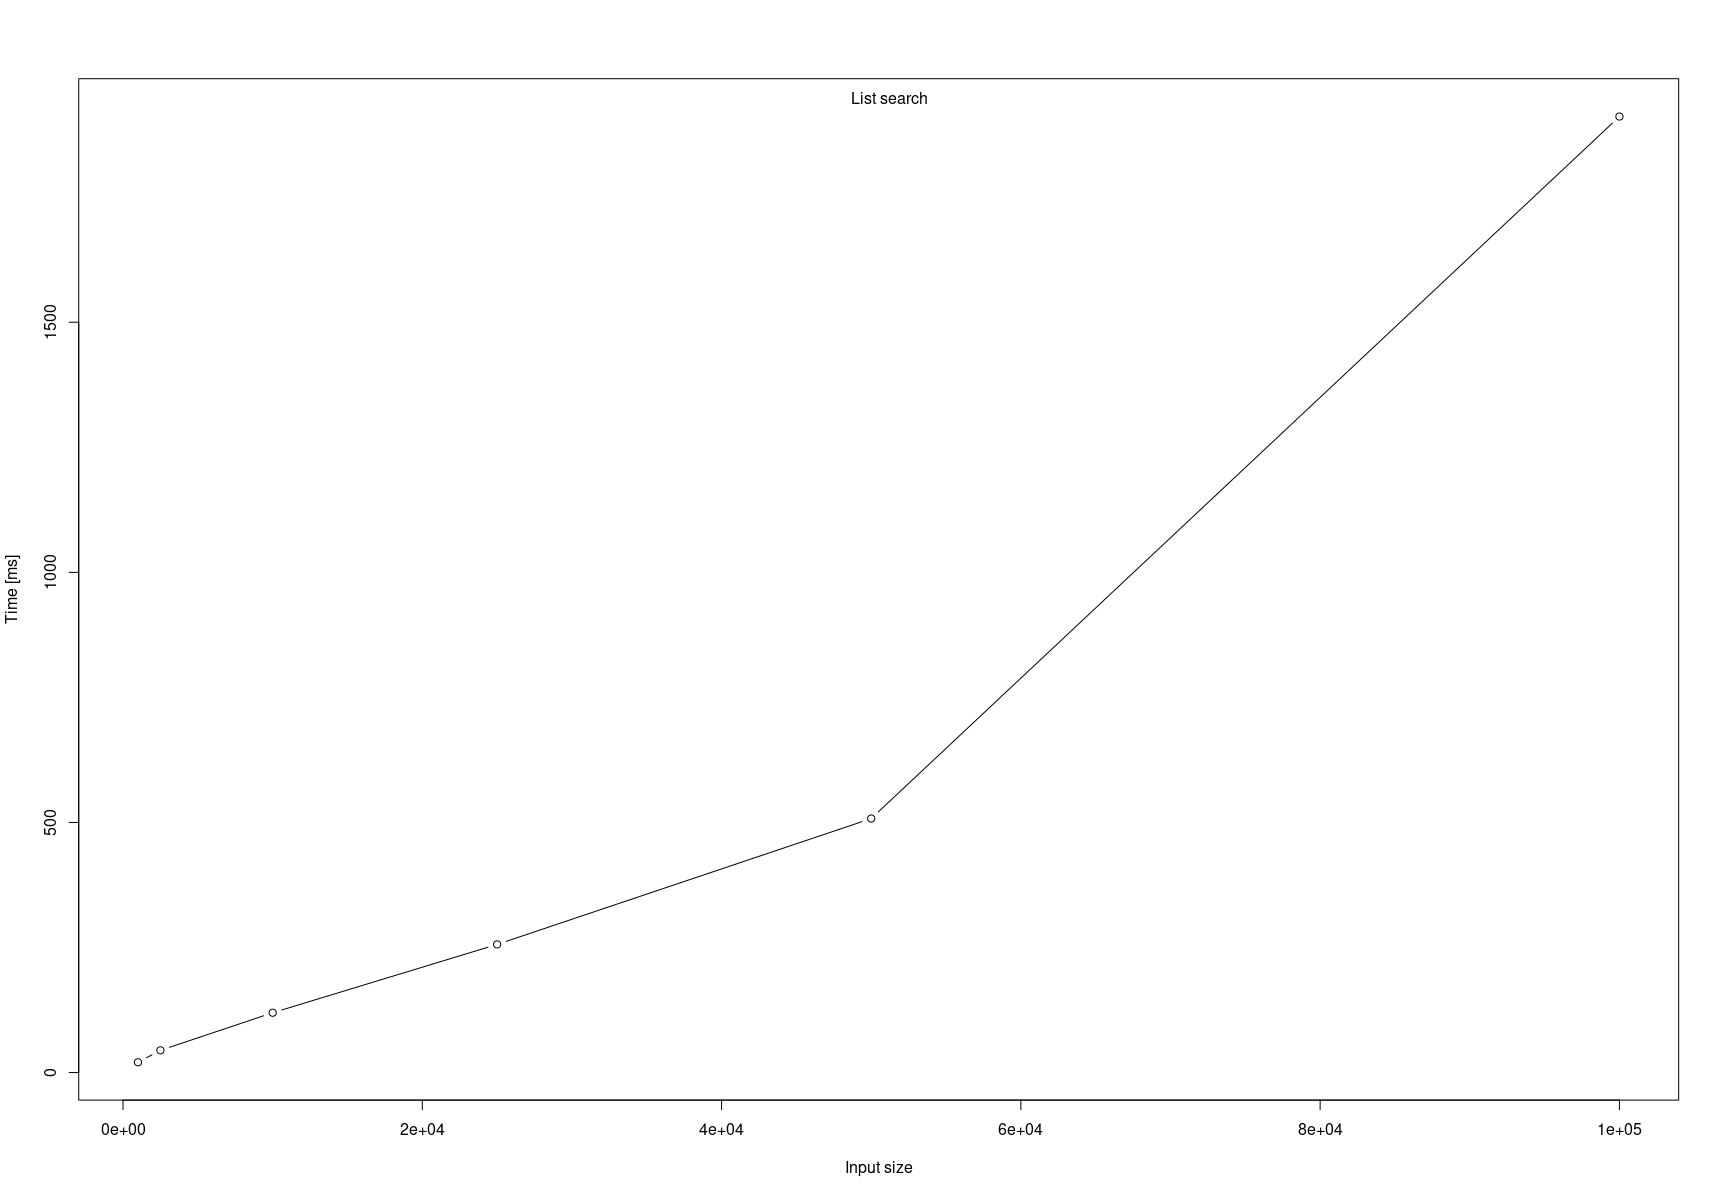
\includegraphics[width=\linewidth]{resources/search_time_list.png}
\end{figure}

\begin{figure}
	\centering
	\caption{Runtime of tree-based search}
	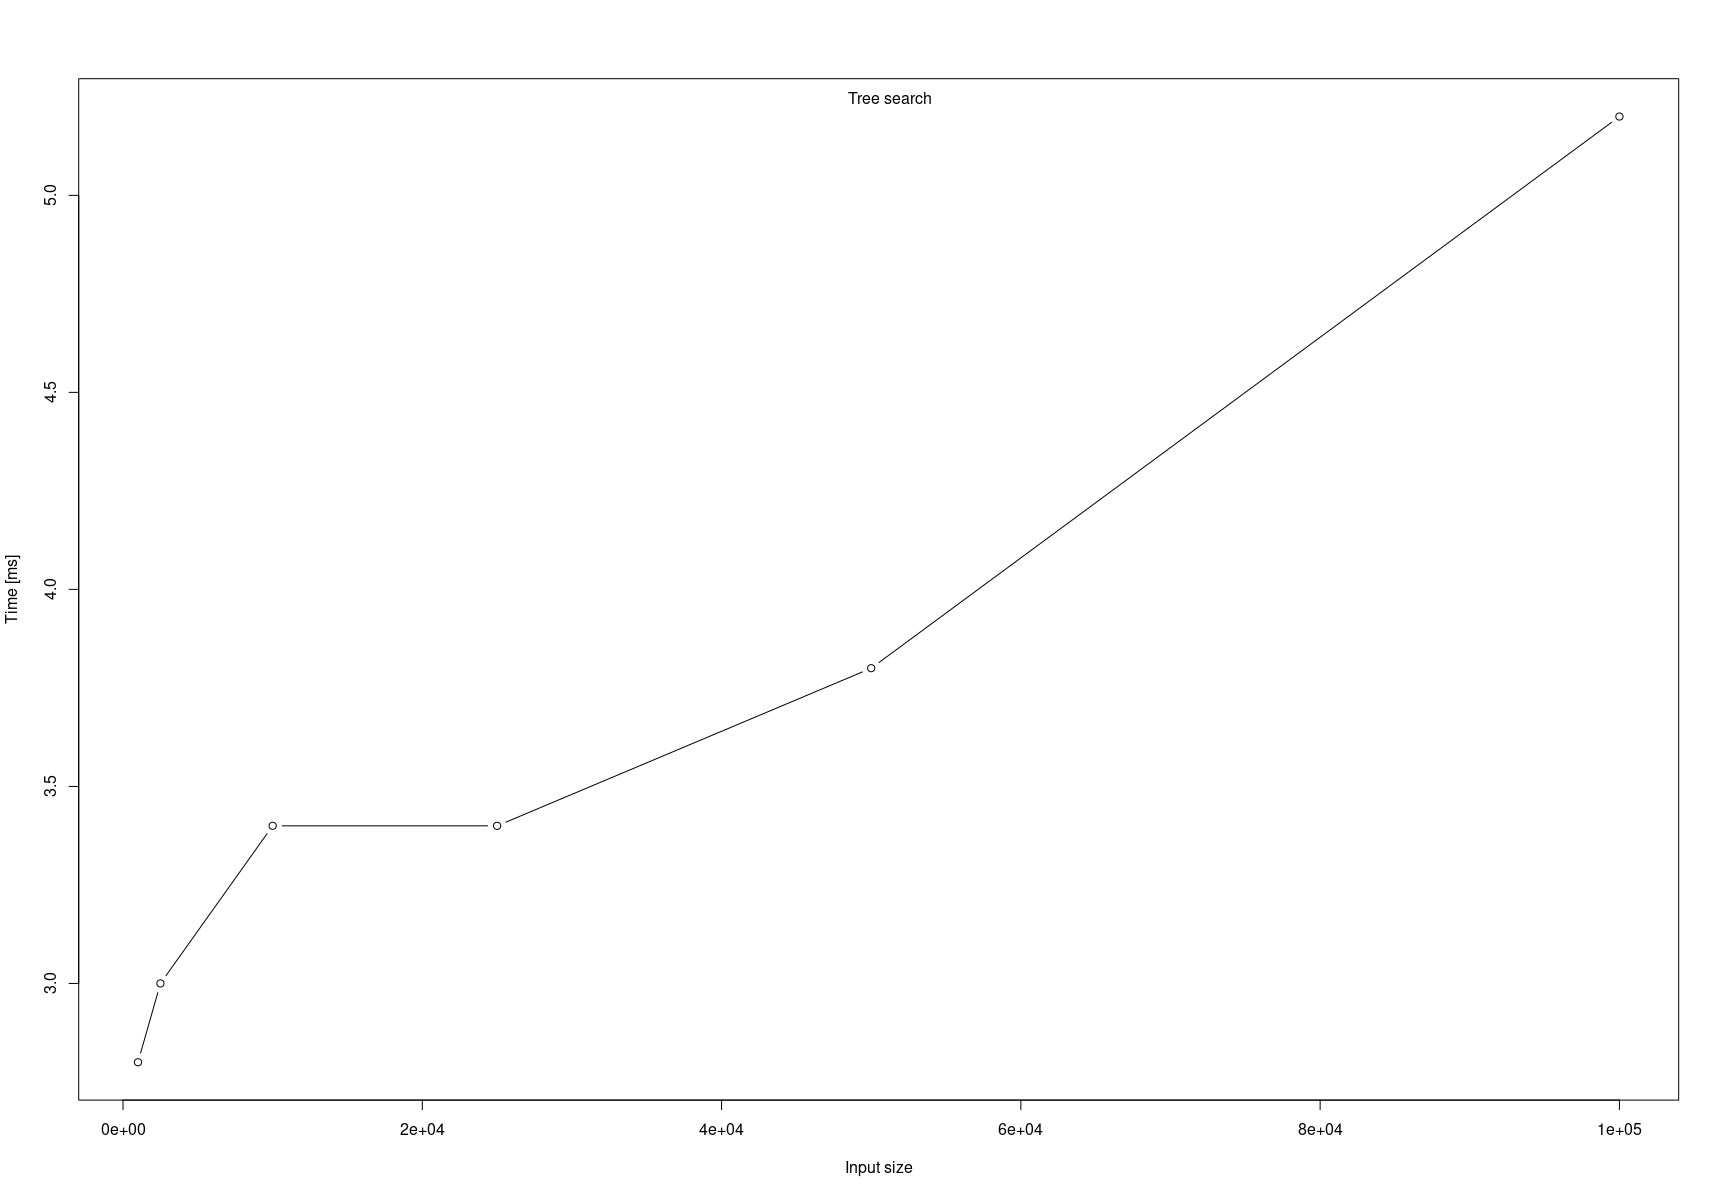
\includegraphics[width=\linewidth]{resources/search_time_tree.png}
\end{figure}

\begin{figure}
	\centering
	\caption{Build-time of KD tree}
	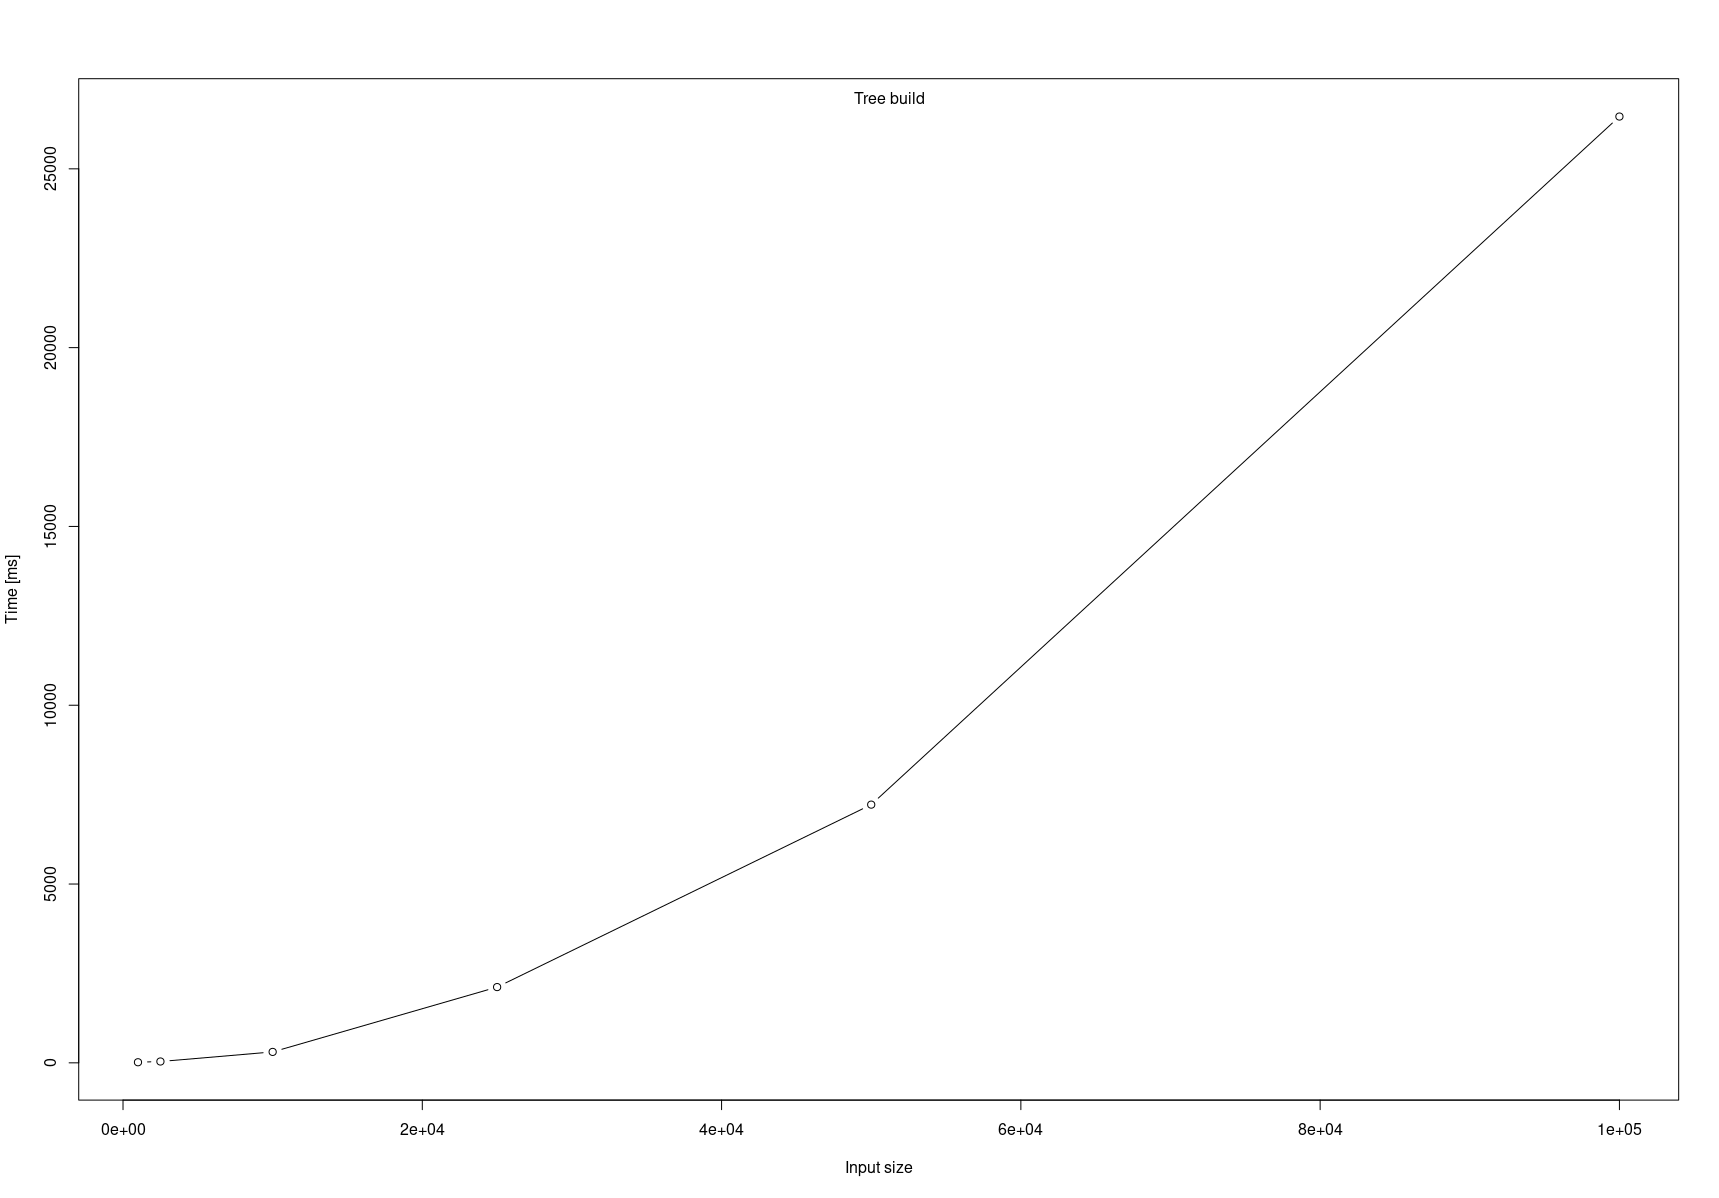
\includegraphics[width=\linewidth]{resources/build_time_tree.png}
\end{figure}

\end{document}
